\documentclass[11pt,a4paper]{report}
\usepackage{marvosym}

\assignment{2}
\group{13}
\students{Mathis Delsart}{/}

\begin{document}

\maketitle

Answer to the questions by adding text in the boxes. You may answer in either \textbf{French or English}. Do not modify anything else in the template.  The size of the boxes indicate the place you \textbf{can} use, but you \textbf{need not} use all of it (it is not an indication of any expected length of answer). \textbf{Be as concise as possible! A good short answer is better than a lot of nonsense!}
%\bigskip

\section{Exercises (5~pts)}

\textit{The following figure assigns a unique letter to each node, and a unique number to each branch. Use it to answer the following questions.}
\begin{center}
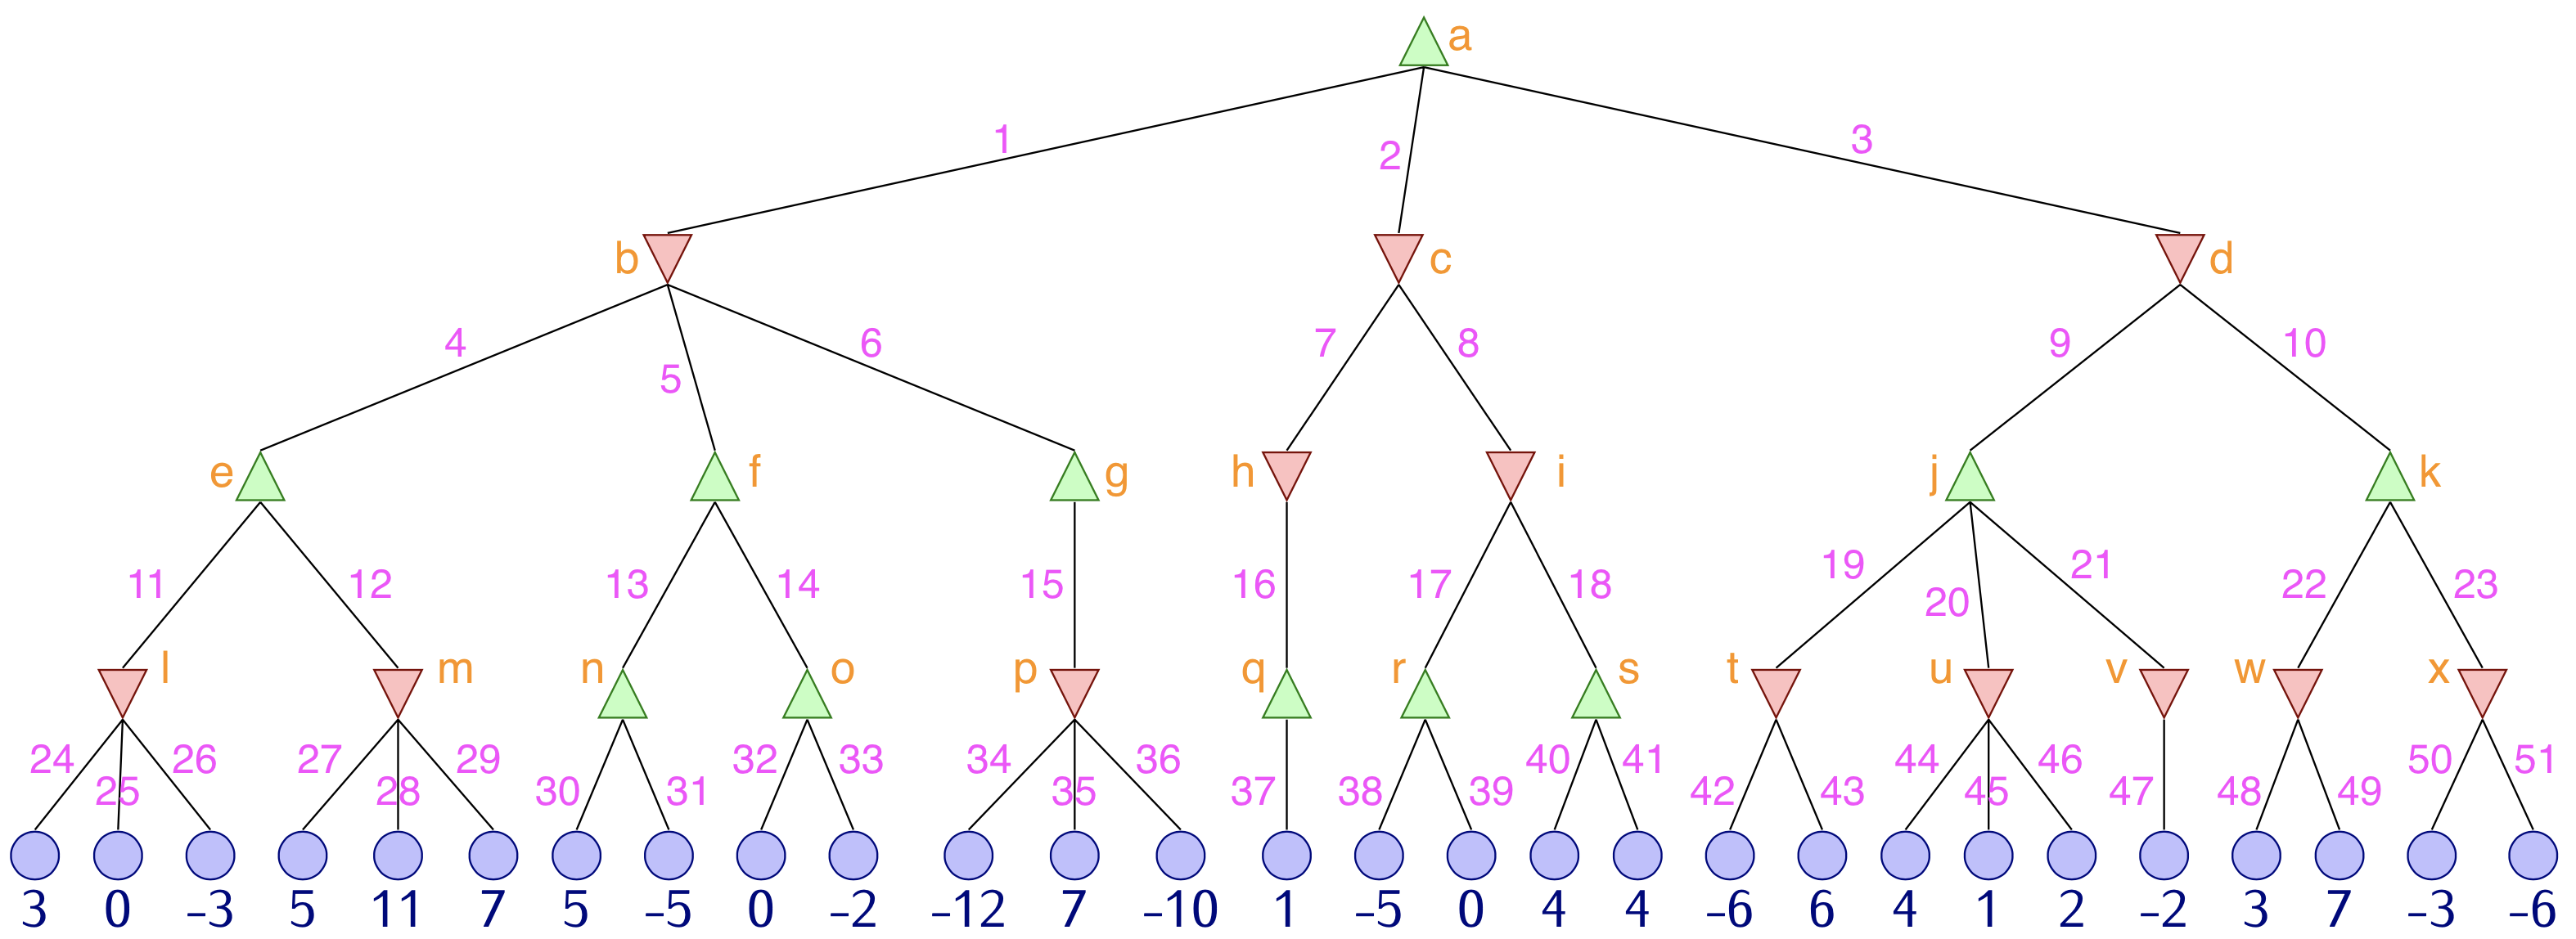
\includegraphics[width=\linewidth]{images/minimax_labelled.png}
\end{center}


\begin{enumerate}
\item Perform the MiniMax algorithm on the following tree, i.e.
      put a value to each node. What move should the root player do? \textbf{(1~pt)}
      
      \textit{Assign a numerical value to each node, and indicate the move (i.e.\! 1, 2, or 3) to perform:}
\end{enumerate}
    % TODO : VERIFIER
      \begin{answers}[3cm]
      \begin{multicols}{5}
      \textbf{a: 1}
      
      \textbf{b: -12}
      
      \textbf{c: 0}
      
      \textbf{d: 1}
      
      \textbf{e: 5}
      
      \textbf{f: 5}
      
      \textbf{g: -12}
      
      \textbf{h: 1}
      
      \textbf{i: 0}
      
      \textbf{j: 1}
      
      \textbf{k: 3}
      
      \textbf{l: -3}
      
      \textbf{m: 5}
      
      \textbf{n: 5}
      
      \textbf{o: 0}
      
      \textbf{p: -12}
      
      \textbf{q: 1}
      
      \textbf{r: 0}
      
      \textbf{s: 4}
      
      \textbf{t: -6}
      
      \textbf{u: 1}
      
      \textbf{v: -2}
      
      \textbf{w: 3}
      
      \textbf{x: -6}
      
      \textbf{Move: 3}
      \end{multicols}
	  \end{answers}



\begin{enumerate}
\item[2.] Perform the Alpha-Beta algorithm on the same tree.
      At each non terminal node, put the successive values of $\alpha$ and
      $\beta$. Cross out the arcs reaching non visited nodes. Assume a
      left-to-right node expansion. \textbf{(1~pt)}
      
      \textit{Indicate the successive $\alpha$ and $\beta$ values of each node in the table below. Separate successive values by a comma (,). Indicate at the bottom the identifiers of the branches that are cut (in increasing order, separated by a comma) (indicate only the branches where the cuts happen, i.e.\!} don't \textit{indicate the branches that are below a cut).}
\end{enumerate}

\begin{answers}[8cm]
      \begin{multicols}{2}
      \begin{tabular}{ccc}
      Node & $\alpha$ values & $\beta$ values\\
      \hline
      \textbf{a} & - $\infty$, -12, 0, 1 &  + $\infty$ \\ 
      \textbf{b} & - $\infty$ & + $\infty$, 5, -12 \\
      \textbf{c} & -12 & + $\infty$, 1, 0 \\
      \textbf{d} & 0 & + $\infty$, 1 \\
      \textbf{e} & - $\infty$, -3, 5 & + $\infty$ \\
      \textbf{f} & - $\infty$, 5 & 5 \\
      \textbf{g} & - $\infty$, -12 & 5 \\
      \textbf{h} & -12 & + $\infty$, 1 \\
      \textbf{i} & -12 & 1, 0 \\
      \textbf{j} & 0, 1 & + $\infty$ \\
      \textbf{k} & 0, 3 & 1 \\
      \textbf{l} & - $\infty$ & + $\infty$, 3, 0, -3 \\
      \textbf{m} & -3 & + $\infty$, 5 \\ 
      \end{tabular}
      
      \begin{tabular}{ccc}
      Node & $\alpha$ values & $\beta$ values\\
      \hline
      \textbf{n} & - $\infty$, 5 & 5 \\
      \textbf{o} & / & / \\
      \textbf{p} & - $\infty$ & 5, -12 \\
      \textbf{q} & 12, 1 & + $\infty$ \\
      \textbf{r} & -12, -5, 0 & 1 \\
      \textbf{s} & -12, 4 & 0 \\
      \textbf{t} & 0 & + $\infty$, -6 \\
      \textbf{u} & 0 & + $\infty$, 4, 1 \\
      \textbf{v} & 1 & + $\infty$, -2 \\
      \textbf{w} & 0 & 1 \\
      \textbf{x} & / & / \\
       &  &  \\
      \end{tabular}
      \end{multicols}
      
\textbf{Cuts: 14, 23, 31, 41, 43}
\end{answers}





\begin{enumerate}
\item[3.] Do the same, assuming a right-to-left node expansion instead.  \textbf{(1~pt)}
\end{enumerate}

\begin{answers}[8cm]
      \begin{multicols}{2}
      \begin{tabular}{ccc}
      Node & $\alpha$ values & $\beta$ values\\
      \hline
      \textbf{a} & - $\infty$, 1 & + $\infty$ \\
      \textbf{b} & 1 & + $\infty$, -10 \\
      \textbf{c} & 1 & + $\infty$, 0 \\
      \textbf{d} & - $\infty$ & + $\infty$, 3, 1 \\
      \textbf{e} & / & / \\
      \textbf{f} & / & / \\
      \textbf{g} & 1 & + $\infty$ \\
      \textbf{h} & / & / \\
      \textbf{i} & 1 & + $\infty$, 4 \\
      \textbf{j} & - $\infty$, -2, 1 & 3 \\
      \textbf{k} & - $\infty$, -6, 3 & + $\infty$ \\
      \textbf{l} & / & / \\
      \textbf{m} & / & / \\ 
      \end{tabular}
      
      \begin{tabular}{ccc}
      Node & $\alpha$ values & $\beta$ values\\
      \hline
      \textbf{n} & / & / \\
      \textbf{o} & / & / \\
      \textbf{p} & 1 & + $\infty$, -10 \\
      \textbf{q} & / & / \\
      \textbf{r} & 1 & 4 \\
      \textbf{s} & 1, 4 & + $\infty$ \\
      \textbf{t} & 1 & 3, -6 \\
      \textbf{u} & -2 & 3, 2, 1 \\
      \textbf{v} & - $\infty$ & 3, -2 \\
      \textbf{w} & -6 & + $\infty$, 3 \\
      \textbf{x} & - $\infty$ & + $\infty$, -3, -6 \\
       &  &  \\
      \end{tabular}
      \end{multicols}
      
\textbf{Cuts: 4, 5, 7, 34, 35}
\end{answers}




\clearpage
\begin{enumerate}
\item[4.] Is there a node ordering that can lead to a more optimal pruning of the tree
(in the sense where the algorithm prunes more branches than in the two other
considered cases)? If no, explain why. If yes, give a new node ordering and the
resulting new pruning.  \textbf{(1~pt)}
      
      \textit{Insert an image below containing the reordered tree, with successive $\alpha$/$\beta$ values indicated next to each node, and where the branches that are cut by the algorithm are crossed out. This may either be an edited version of \texttt{minimax\_empty.png} (using paint, gimp, etc.), a photograph of a drawing you made by hand, etc. In any case, the image must be \textbf{clear} in order to be graded.}
\end{enumerate}

\begin{answers}[8cm]
\footnotesize{\textbf{Yes}, there is a \textbf{node ordering} that leads to a more optimal pruning of the tree. \\
\textbf{For the maximizing player}, nodes should be ordered in \textbf{decreasing order}, ensuring the best node is explored first.
Conversely, \textbf{for the minimizing player} (the opponent), nodes should be ordered in \textbf{increasing order}, prioritizing their best move. \\
The \textbf{goal of this ordering method} is to \textbf{always visit the best move available for the player currently taking their turn}.}
\begin{center}
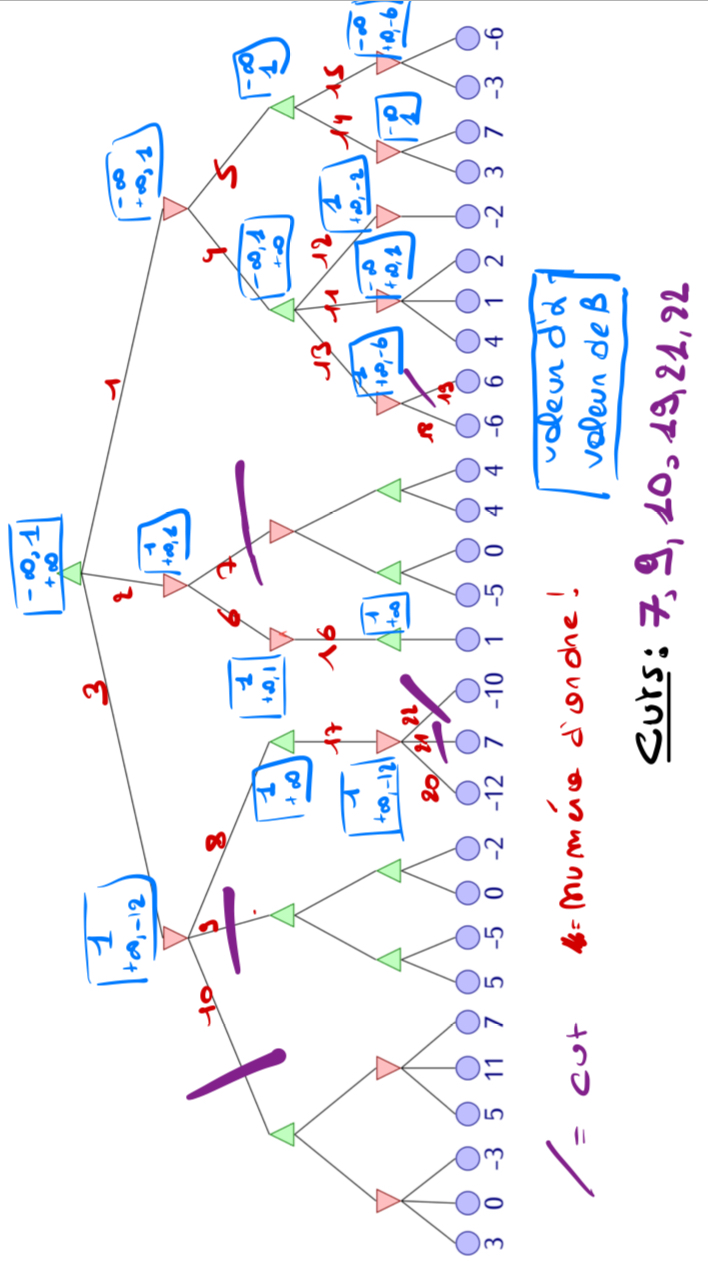
\includegraphics[angle=-90,scale=.22]{images/reorderedNodes_Alphabeta.png}
\end{center}
\end{answers}




\begin{enumerate}
\item[5.] How does Alpha-Beta need to be modified for games with more than two players? \textbf{(1~pt)}
\end{enumerate}

\begin{answers}[9cm]
\small{To modify Alpha-Beta for games with more than two players, the basic Minimax algorithm must first be \textbf{generalized into the MaxN algorithm}. In MaxN, players take turns making moves and aim to \textbf{maximize their perceived returns, while being indifferent to the returns of other players}. At the leaf nodes, the evaluation function is applied, now \textbf{returning an N-tuple of values}, where N is the number of players. Each component corresponds to the estimated merit of the position for one of the players. \textbf{When it's player i's turn, they choose the i-th component of the N-tuple from a child node that maximizes this value}. \\

Additionally, the pruning principle needs to be generalized, thus adapting the Alpha-Beta algorithm. It's crucial to establish \textbf{upper bounds for the total sum of components of each value tuple}, as well as \textbf{lower bounds for each individual component}. Ensuring that \textbf{each individual value cannot exceed a certain lower limit}, typically \textbf{set at zero}, is also necessary to avoid unbounded values that could lead to excessive computations.

Now, there are \textbf{two forms of pruning}. The first form, called \textbf{immediate pruning}, occurs when \textbf{player i is to move} and the \textbf{i-th component of one of its children equals the upper bound on the sum of all components}. In this case, \textbf{all remaining children can be pruned} because \textbf{no child's i-th component can exceed the upper bound on the sum}. Then, there is \textbf{shallow pruning}, a more complex situation. For example, in a three-player game, evaluating a node involves establishing upper and lower bounds on the remaining components, depending on the player involved. If the upper bound of a child is lower than the lower bound of the previous child, the latter and its children can be pruned. \\

\underline{\textbf{Source:}} $\href{URL}{https://faculty.cc.gatech.edu/~thad/6601-gradAI-fall2015/Korf_Multi-player-Alpha-beta-Pruning.pdf}$}

\end{answers}




\clearpage
\section{Shobu (35~pts)}
\medskip

\subsection{Alpha-Beta agent (4 points, to be submitted on Inginious)}
\medskip


\subsection{Monte-Carlo Tree Search agent (5 points, to be submitted on Inginious)}
\medskip


\subsection{Warm-up questions (3 points)}
\begin{enumerate}
\item[1.] What is the branching factor at the start of the game? What is the mean empirical branching factor? (The branching factor is considered here as the number of possible moves that a player can do from a given state). \textbf{(1 point)}
\end{enumerate}

\begin{answers}[5cm]
\small{The game Shobu is characterized by its \textbf{symmetry about the board}, meaning the initial moves for players on both boards are equivalent.
Therefore, we'll \textbf{analyze a passive move on one board and an aggressive move on the other, multiplying the result by 4} to account for this symmetry for both types of moves. \\

On one of the boards: vertical move (1 square) $\Rightarrow 4 \times 4 = 16$, vertical move (2 squares) $\Rightarrow 4 \times 4 = 16$, diagonal move (1 square) $\Rightarrow 2 \times 3 \times 3 = 18$, diagonal move (2 squares) $\Rightarrow 2 \times 2 \times 2 = 8$.

Thus, for the start of the game only, \textbf{$b = 4 \times (16 + 16 + 18 + 8) = 232$}. \\
We \textbf{confirmed the result using "len(game.actions(game.initial))"}, and \textbf{found the same result ($= 232$)}. \\

To \textbf{estimate the mean branching factor}, we \textbf{simulated 100,000 games randomly. \\
For each game}, we \textbf{calculated the branching factor and then took the average of these values}. By the \textbf{law of large numbers}, we observe that \textbf{the result converges} to \textbf{$b = 85$}.}

\end{answers}



\begin{enumerate}
\item[2.] What would be one (of the many) drawbacks of the simple heuristic that is imposed for the basic alpha-beta agent above? \textbf{(1 point)}
\end{enumerate}

\begin{answers}[10cm]
One of the main drawbacks of this simple heuristic is its profound \textbf{lack of knowledge about the game}. \\

By solely considering the minimum number of pieces on the boards, it \textbf{completely overlooks crucial aspects}. \\

It fails to take into account \textbf{imminent threats}, \textbf{defensive} and \textbf{offensive structures}, and \textbf{does not differentiate} between \textbf{advantageous or disadvantageous situations} due to the \textbf{absence of consideration} for the \textbf{quality of piece placement}.
By example, it does not take into account the \textbf{central positions} (the 4 middle squares) \textbf{as advantageous} and it makes \textbf{no distinction} in strategy between \textbf{\textit{Home} and \textit{Opponent} boards}. \\

Additionally, it lacks the ability to \textbf{distinguish between different game states} that may have \textbf{the same minimum number of pieces} and thus the \textbf{same score}, resulting in \textbf{suboptimal decision-making}. \\

\textbf{\textit{A good heuristic try to give a different score for each single state !}} \\

See \textit{question \textbf{2.4}} for the optimisation of this simple heuristic.
\end{answers}


\begin{enumerate}
\item[3.] Considering the Monte-Carlo Tree Search algorithm, what is the hypothesis supporting the use of random simulation to estimate the win rate? Is this hypothesis always valid? \textbf{(1 point)}
\end{enumerate}

\begin{answers}[15cm]
The \textbf{fundamental assumption} underlying the \textbf{use of random simulations} in the MCTS algorithm is the \textbf{law of large numbers}. This mathematical law states that \textbf{with a sufficiently large number of simulations}, the \textbf{estimated win rate should converge to the true win rate of the game}. \\

Mathematically, this law can be expressed as follows:
\[
\lim_{n \to +\infty} \mathbf{P} \left( \left| \overline{X}_n - \mu \right| > \varepsilon \right) = 0 \quad \forall \varepsilon > 0
\]

In this formula, \(n\) represents \textbf{the number of samples (simulations)} performed, \(X_i\) is a random variable representing the \textbf{result of the \(i\)-th simulation} (where \textbf{1 indicates a win}, \textbf{-1 a loss and 0 a draw}), \(\overline{X}_n\) is the \textbf{average of the simulation results}, \(\mu\) is the \textbf{mathematical expectation of \(X_i\)}, and \(\varepsilon\) is a \textbf{small margin allowed from \(\mu\)}. \\

It is important to note that for the law of large numbers to be applicable, a \textbf{sufficiently large number of samples must be used}. Otherwise, the \textbf{estimated win rate may not be representative of the true win rate of the game}. \\

However, \textbf{this hypothesis is not always valid}, particularly in games where the \textbf{game tree is too large to adequately sample with random simulations alone}. In the game \textit{Shobu}, random moves do not represent well an actual playout of the game. This is due to the complexity and strategic depth of the game, which random simulations fail to capture. Another case where this assumption is invalid is when there are \textbf{very abrupt and extreme changes in state evaluations}. In this scenario, the convergence of the sample mean to the true mean can be compromised. In such cases, the effectiveness of the MCTS algorithm may be limited.

\end{answers}


\newpage
\subsection{Description of your agent (8 points)}
Describe in the boxes below what you have implemented for your contest agent. You can also mention things that you tried and did not work but focus on what you have submitted in the end.

\begin{answers}[21cm]
\subsubsection{Algorithm Used}
We implemented the \textbf{MiniMax algorithm with alpha-beta pruning}. This choice was made after comparing the two basic versions (AlphaBeta and MCTS), and observing that MCTS performed poorly in the Shobu game. Moreover, \textbf{MiniMax seemed simpler to understand and optimize}.

\subsubsection{Heuristic}

Here are the features considered in our heuristic guiding our tree search. Everything detailed below was done for both players. When something is \textbf{advantageous for the AI}, we \textbf{assign a positive score}, while if it's \textbf{advantageous for the opponent}, we \textbf{assign a negative score}. This allows MiniMax to \textbf{maximize the AI's score and minimize the opponent's score} during the search.

\begin{itemize}
    \item \textbf{\textit{Material advantage}}
\end{itemize}
We considered the \textbf{minimum number of pieces remaining on either board}, as well as the \textbf{total number of pieces remaining on all four boards}.

\begin{itemize}
    \item \textbf{\textit{Positional advantage}}
\end{itemize}
We \textbf{favored central positions} (the 4 center squares). A \textbf{bonus} is also given if these \textbf{central positions are reached on the opponent's boards}, as actions can still be taken on both opponent boards, allowing \textbf{more attacking options}. A \textbf{bonus} is also awarded if the \textbf{central position is on the opponent's side} (thus, 2 out of 4 squares), as it's a strategically advantageous attacking position.

\begin{itemize}
    \item \textbf{\textit{Mobility advantage}}
\end{itemize}
We simply calculated the \textbf{number of possible moves for a state for both players}.

\begin{itemize}
    \item \textbf{\textit{Strategic advantage}}
\end{itemize}
This feature encompasses several sub-features, all representing strategic advantages through positioning. We assign a score to \textbf{stones located on the opponent's side} (position > 7 for white player), favoring attacks. We also give a significant bonus for a \textbf{specific attacking position} that we found interesting to implement. For example, if the white player is at position 14 (resp. 13) and there are opponent stones on squares 13 and 15 (resp. 12 and 14), the win percentage for white player in this case is very high because it's a \textbf{strategically crucial position}. A \textbf{high score was assigned to this special position}. And smaller scores were still assigned if there's only one opponent stone on each side of the white stone. The last strategic feature \textbf{assigns a score to stones placed between two opponent stones in the same direction}. This position is interesting because the \textbf{player's stone can push both opponent stones, but the opponent stones cannot push the player's stone}! \\

To ensure that all features are on \textbf{the same scale}, we searched for the maximum and minimum values each feature can take, and applied this formula: \textbf{$valueScaled = \frac{valueNotScaled - minValue}{maxValue - minValue}$}. This yields scores \textbf{between 0 and 1}.

\end{answers}

\begin{answers}[23cm]

We then \textbf{manually determined the weights for each feature to obtain the best possible evaluation}. We had considered \textbf{dynamically adjusting the weights using a deep learning algorithm}, but we lacked the time (and talent) to implement it.

The chosen weights are \textbf{0.50, 0.25, 0.20, and 0.05, respectively, for material advantage, positional advantage, strategic advantage, and mobility advantage}.

\subsubsection{Node Rearrangement}

We initially implemented a \textbf{complete node rearrangement function using the evaluation function}. However, the \textbf{computation time was excessively high}, so we abandoned the idea and opted for a less optimal but much more accessible strategy in terms of computation time. This strategy is to \textbf{place all actions leading to pushing an opponent stone out of one of the boards first in the action list}. This feature doesn't make much sense initially, but eventually, it allows for \textbf{more pruning using this node rearrangement function because nodes likely to lead to more advantageous game states for the player are explored first by the algorithm}.

\subsubsection{Iterative Deepening}

Since \textbf{time was the constraint of the algorithm} (one game = 300 seconds for our agent), we opted for an \textbf{iterative deepening algorithm while keeping track of the best action from the previous iteration to place this action first in the action list in the next iteration}. This technique is a node rearrangement technique as discussed in the previous section. It's often referred to as a \textbf{\textit{killer move heuristic}}. The first depth used is 1 and then the depth in increased by 1 at each iteration. \textbf{If the maximum time allowed for an iteration is reached, then the algorithm stops and returns the best action found among all iterations performed}. With this algorithm, we can \textbf{avoid for sure the time-out}, provided that we have our maximum time allowed for a single iteration not too long. \textbf{We estimate it at 15 seconds}.

\subsubsection{Transposition Table}

We implemented a \textbf{transposition table} taking into account the symmetries of the game discussed in the next section.

The transposition table allows us to \textbf{retrieve the evaluation of a state if this game state has already been encountered and evaluated before}. To store the state in memory, we \textbf{hash it into a unique string by scanning from left to right and bottom to top of the board}. A "." represents an empty square, "o" represents a white stone, and "x" represents a black stone. The initial state of the game is represented as follows: "oooooooo................xxxxxxxxxxxxxxxx................oooooooo".

This improvement \textbf{consumes a lot of memory} but is \textbf{very useful for avoiding recalculation of many parts of the tree already calculated before}.

\subsubsection{Shobu Game Symmetry}

The Shobu game exhibits a \textbf{lot of symmetry}. Therefore, we created a class that takes a \textbf{game state hashed as input} and \textbf{outputs whether a symmetry of this state already exists in the transposition table}. If a symmetry exists, then the evaluation of the state is already known and doesn't need to be recalculated! This improvement is therefore only used with the transposition table discussed in the previous point.

\end{answers}

\begin{answers}[23cm]

We considered \textbf{various symmetries}. The simplest are the \textbf{rotations of the 4 boards individually}. Each board \textbf{can rotate at 90° / 180° or 270°}. \textit{Note that all boards must rotate by the same amplitude}. There are also \textbf{switches between the two Home boards, the two Opponent boards, or even both switches simultaneously}. \textit{Note that Home and Opponent boards cannot be modified between each other, as this would change the game properties}. Additionally, for each board taken individually, there are \textbf{vertical, diagonal, and inverse diagonal symmetries} (horizontal already accounted for during the 180° rotation). The last symmetry is the \textbf{color change of stones}. \texit{Note that in this symmetry, the evaluation value is inverted (17 becomes -17 and vice versa)!}

\texit{This improvement allows us to \textbf{avoid a large part of the search tree because symmetries in this game are omnipresent due to the idea of the 4 distinct boards in the game}}. \\

\subsubsection{Features Ideas Not Implemented}

\begin{itemize}
    \item \textbf{\textit{Quiescent search}}
\end{itemize}

In our iterative deepening algorithm, we tried to implement \textbf{quiescent search to enhance the search process}. Quiescent search is particularly beneficial for \textbf{resolving the horizon effect problem}. This technique \textbf{extends the search to capture tactical positions where the game is relatively stable, ensuring that the evaluation captures critical tactical threats and captures}.

\texit{Unfortunately, we have not observed good results. Either we made errors in the implementation, or this feature is not useful for the game Shobu.}

\begin{itemize}
    \item \textbf{\textit{EndGame Lookup table}}
\end{itemize}

We had considered implementing a \textbf{lookup table for endgames} as it's often used in chess since endgame moves are often known because the \textbf{branching factor is much smaller}. This would have allowed us to save a lot of time and \textbf{enable deeper searches in the middle of the game}.

\texit{However, we didn't do it because there was almost no documentation on this topic for the Shobu game, making it practically impossible.}

\end{answers}

\newpage
\subsection{Comparison of agents (5 points)}
Describe here the comparison of the different agents: random, Alpha-Beta, MCTS and your agent (and others if you want!). Remember that it should be a statistical comparison. Describe how you compare the agents. Draw some observations and conclusions based on the results you have obtained.

\begin{answers}[20cm]

\subsubsection{Introduction}
For the comparison of our four agents, we conducted three tests that we consider relevant. For each of these tests, we will present the results (table or graphs) and provide interpretations of the results.

\subsubsection{Test 1: Win Rate}
In this test, each agent played against every other agent. This test was conducted under fair conditions, meaning each agent played 10 games, with 5 as the white player and 5 as the black player. Figure \ref{fig:HeapMap_WinRate} shows the results in the form of a heatmap.

\begin{center}
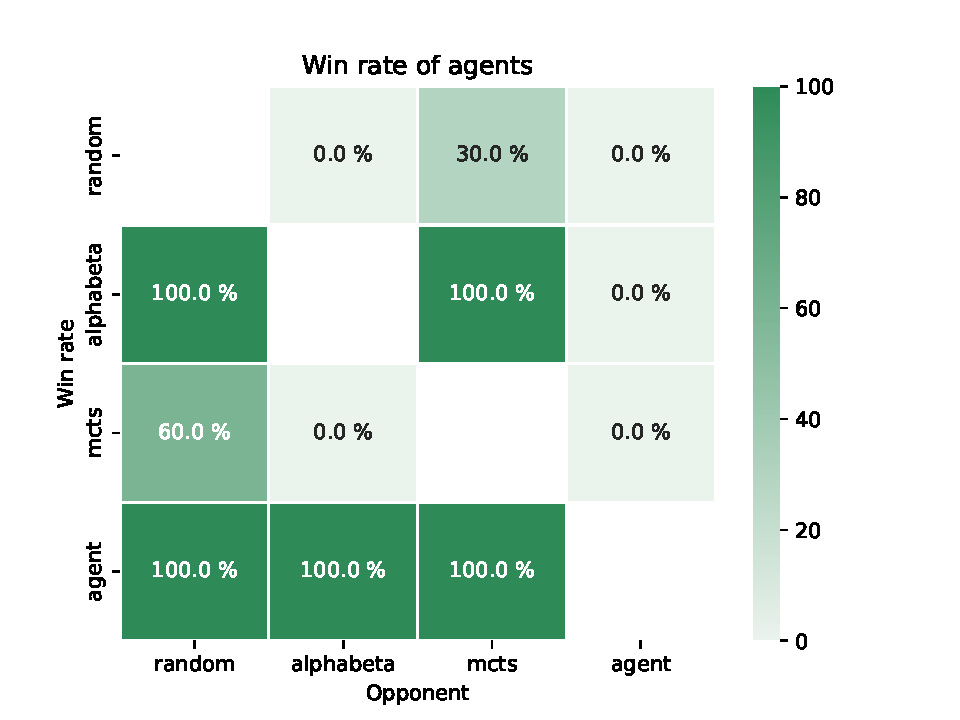
\includegraphics[width=0.60\textwidth]{images/graphs/WinRate.pdf}
\captionof{figure}{Win Rate HeapMap}
\label{fig:HeapMap_WinRate}
\end{center}

We observe that our agent emerges victorious in all games against the other agents. The AlphaBeta agent, on the other hand, suffers defeat in all games against our agent. Additionally, the MCTS agent only manages to win 60 percents of the games against the random agent, indicating poor performance in the Shobu game. This could be attributed to the fact that MCTS simulations are too slow, thereby limiting its ability to explore a substantial number of nodes within the given time frame. Consequently, it fails to gather sufficient information to make informed decisions, akin to the random agent's approach. Thus, it's not surprising that its win rate is relatively low. The Alphabeta (and thus our Contest agent as well) is significantly superior to MCTS because Shobu is a game with complete information, and Alphabeta's search is guided by a heuristic. These two conditions make MCTS perform poorly in such scenarios (without notable improvements).

\end{answers}

\begin{answers}[23cm]

\subsubsection{Test 2: Execution Time}
For this test, we analyzed the execution time per move for each agent when playing against a random agent and against themselves. This test also allows us to observe, for each agent, the number of moves required to finish the game against a random agent and against itself. We did not have the random agent play against itself because it is not very meaningful, and we limited the maximum number of moves to 100 for MCTS as it acts almost like a random agent and could technically make an infinite number of moves. Figure \ref{fig:LineChart_ExecTime} shows the results obtained in graphical form.

\begin{figure}[H]
    \centering
    \hspace{0cm}
    \begin{subfigure}[b]{0.50\textwidth}
    \centering
    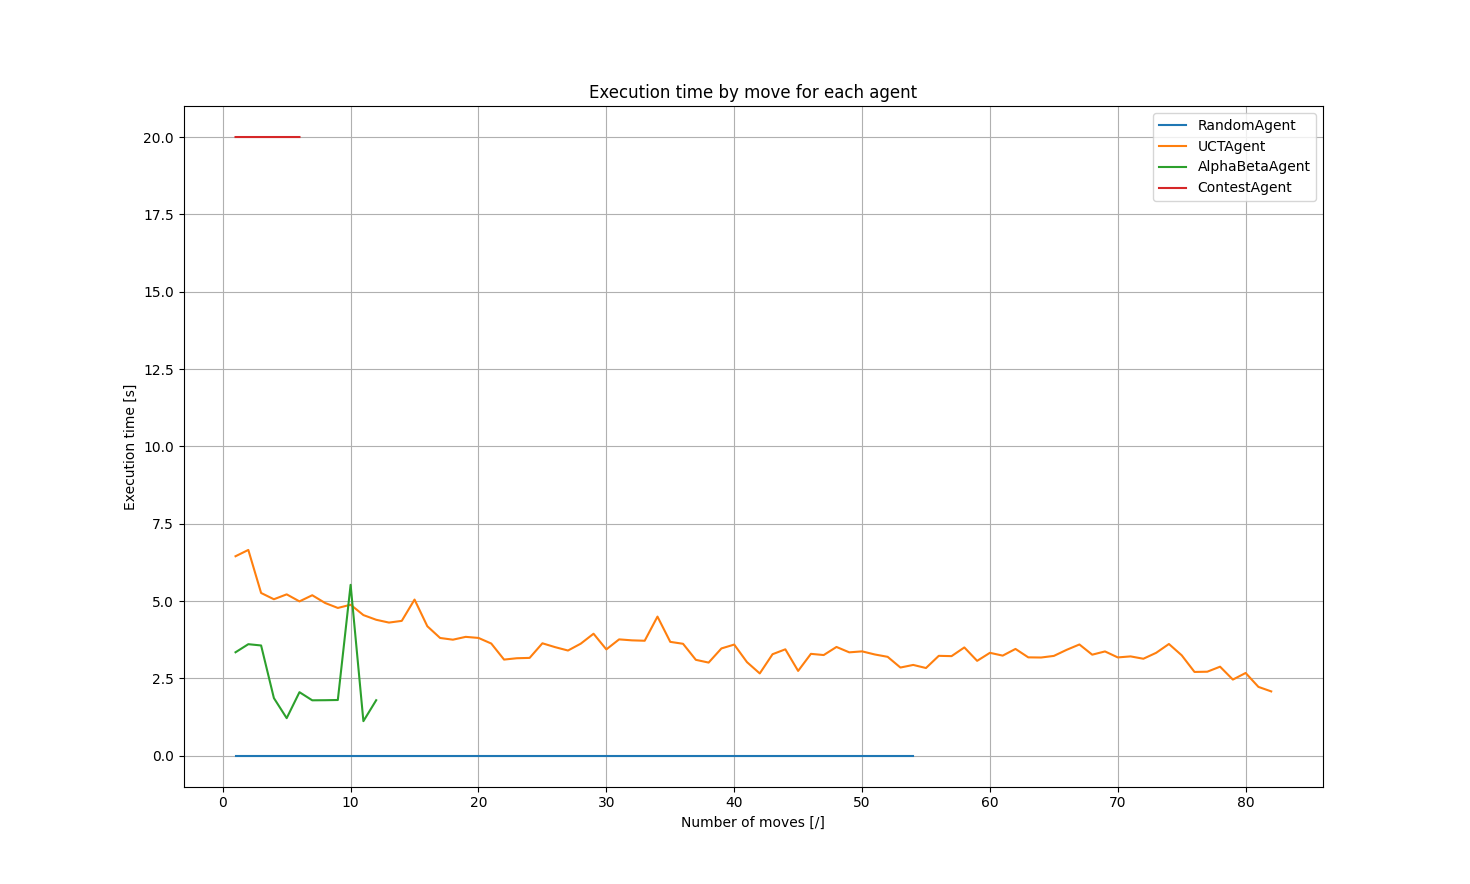
\includegraphics[width=\textwidth]{images/graphs/TimeExecAgainstRandomAgent.png}
    \caption{Against Random Agent}
    \label{fig:ExecTime_Random}
    \end{subfigure}
    \hspace{0cm}
    \begin{subfigure}[b]{0.45\textwidth}
    \centering
    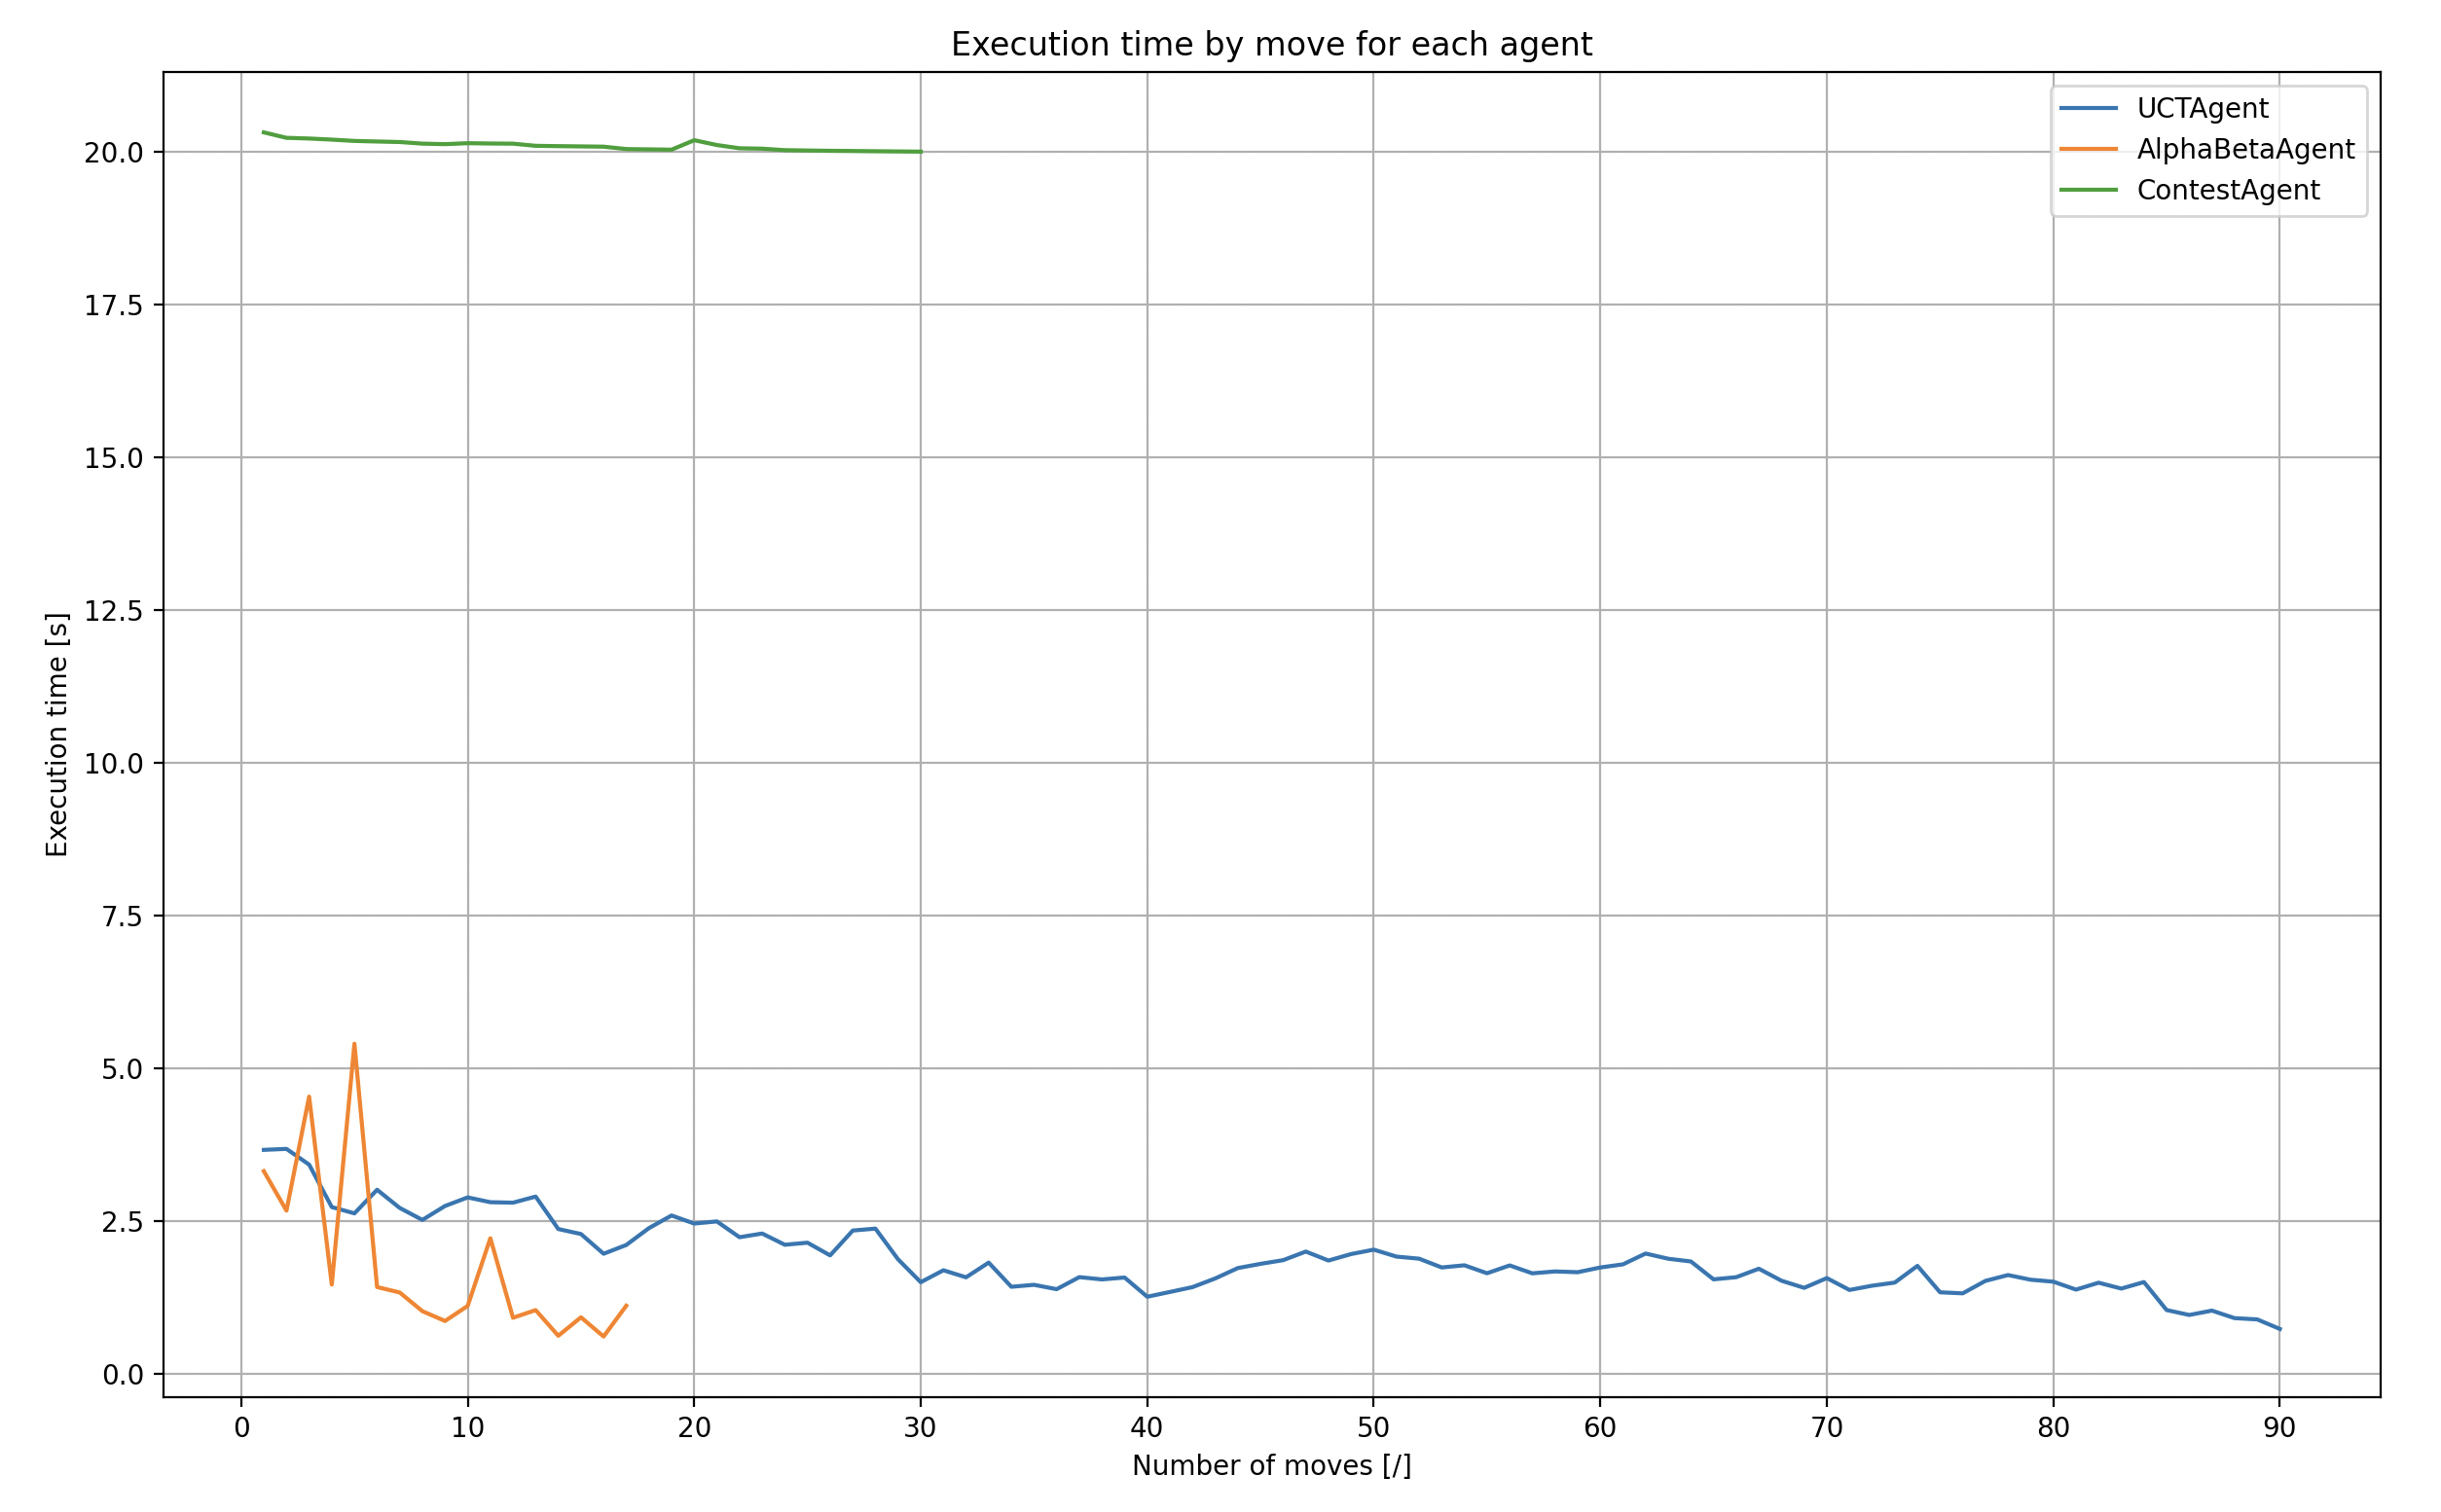
\includegraphics[width=\textwidth]{images/graphs/TimeExecAgainstAgent.png}
    \caption{Against Themselves}
    \label{fig:ExecTime_Agent}
    \end{subfigure}
    \caption{Execution Time by Move for Each Agent}
    \label{fig:LineChart_ExecTime}
\end{figure}

\begin{itemize}
    \item \textbf{\texit{Interpretation of Figure 2.a}}
\end{itemize}
We can observe that the execution time of our Contest agent is constant at 20 seconds, which is normal as it is the allocated time limit per move that we have set for maximum calculation time. We can also see that the MCTS agent is very slow to converge as it takes more than 80 moves to finish the game compared to less than 60 moves for the Random agent. The execution time for the Random agent is constant at 0 seconds because it directly returns a random legal action, so the calculation time is negligible. The last significant observation here is the comparison of the number of moves to finish the game against the Random agent for our agent and for the AlphaBeta agent. The AlphaBeta agent finishes the game in a higher number of moves, demonstrating that our agent plays better and finds optimal moves more easily to finish the game quickly.

\begin{itemize}
    \item \textbf{\texit{Interpretation of Figure 2.b}}
\end{itemize}
We observe that MCTS does not converge because it reaches the limit of 100 moves allowed for the test. The execution time of our agent remains constant at 20 seconds, as explained in the previous section. We can also see that the number of moves in the game is lower for the AlphaBeta agent compared to our agent. This is entirely normal because our agent strives to develop strategies, to position itself in the center, whereas the AlphaBeta agent simply aims to eliminate pieces without considering its positioning. Consequently, it finishes games more quickly, but it also takes a considerable risk as it never adopts a defensive strategy; it only attacks.

\end{answers}

\begin{answers}[23cm]

\subsubsection{Test 3: Explored Nodes}
For this third test, we calculated the number of nodes explored by each agent when playing against a random agent and against itself. Additionally, we took into account the number of moves in the game to demonstrate the number of nodes explored per move. The following figure \ref{fig:NodeExplored} shows the results obtained.

\begin{center}
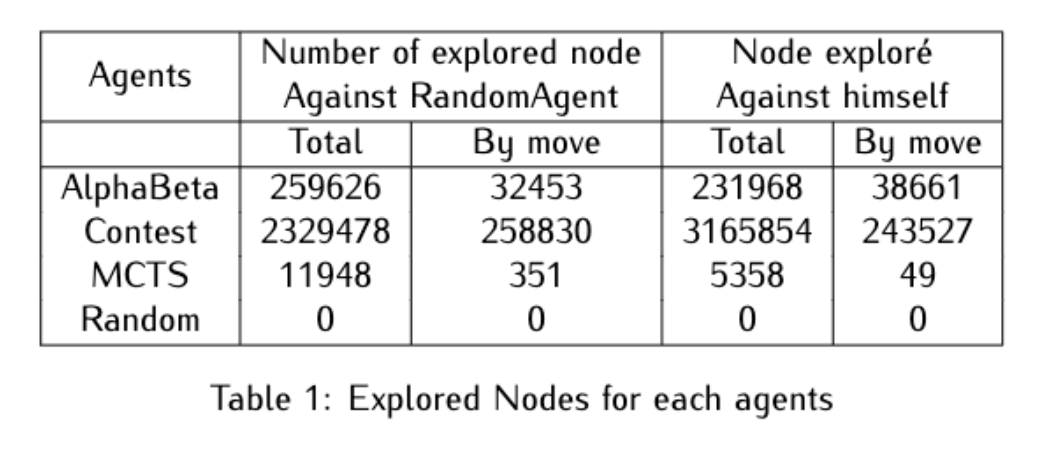
\includegraphics[width=0.60\textwidth]{images/graphs/ExploredNodesTable.png}
\captionof{figure}{Explored Nodes Table}
\label{fig:NodeExplored}
\end{center}

We observe that our agent explores many more nodes than the other agents, which could contribute to its ability to make more informed decisions and therefore achieve better results in the game. The AlphaBeta agent explores a significant number of nodes, but it remains much lower than our Contest agent. The MCTS agent, on the other hand, explores very few nodes due to the slowness of its simulations, which may limit its ability to achieve satisfactory results within a reasonable timeframe. Additionally, the Random agent does not explore any nodes and simply makes random decisions, that's why it's very bad. Thus, the number of nodes explored plays a crucial role in the quality of decisions made by each agent and affects their speed of convergence towards optimal or near-optimal solutions in the game.

\subsubsection{Conclusion}
These three tests demonstrate that our agent outperforms the MCTS, AlphaBeta, and Random agents, which is not surprising since they are basic algorithms without improvements. Our agent is much slower to maximize calculation time but is more optimal in its decision-making. It also explores many more nodes than the other agents, showing that it acquires better knowledge of the search tree with each move.

\end{answers}

\subsection{Contest (10 points, to be submitted on Inginious)}

\end{document}